\subsection{Prueba de rendimiento}
Esta prueba se realiza una vez que hechas las modificaciones como producto de las pruebas unitarias, de integración y de sistema.
\subsubsection{Objetivo de la prueba}
Verificar el uso del GPU. 
\subsubsection{Herramientas utilizadas durante la prueba}
\textit{Profiler de Unity.}
\subsubsection{Aplicación de la prueba}
Esta prueba inicia desde el menú principal y con la herramienta \textit{profiler} se 
observa el desempeño del GPU de la maquina al simular el juego. La ventaja de utilizar 
\textit{Profiler} es que indica que elementos de la escena son los que están 
consumiendo un determinado porcentaje del GPU. En las figuras 
\ref{fig:MenuSelectionprofiler}, \ref{fig:CutSeceneprofiler} y 
\ref{fig:LevelProfiler} se muestran los resultados de la 
herramienta \textit{Profiler}.
\begin{figure}
  \centering
  
   \subfigure[Vista general del uso del GPU.] {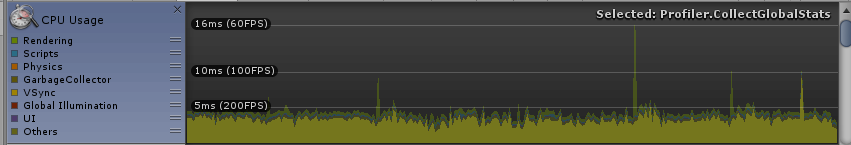
\includegraphics[width=0.6 \textwidth]
   {04ResultadosObetnidos/imagenes/ProfilerMenuselector01.png}}
   
        \subfigure[Desglose de los porcentajes del uso del GPU] {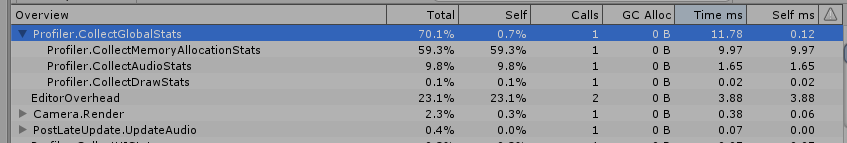
\includegraphics[width=0.6 \textwidth]{04ResultadosObetnidos/imagenes/ProfilerMenuselector02.png}}
        
        \subfigure[Desglose de los porcentajes del uso de memoria] {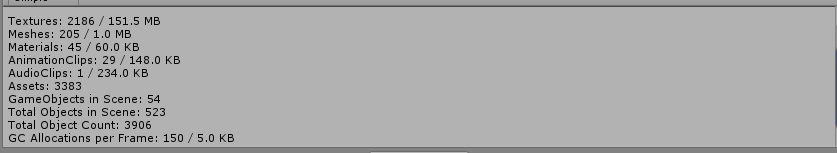
\includegraphics[width=0.6 \textwidth]{04ResultadosObetnidos/imagenes/ProfilerMenuselector04.png}}
  \caption{Resultados de la herramienta \textit{profiler} al analizar el menú de        
  seleccion.}
  \label{fig:MenuSelectionprofiler}
\end{figure} 

\begin{figure}
  \centering
  
   \subfigure[Vista general del uso del GPU.] {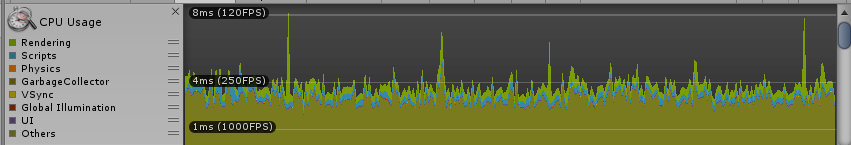
\includegraphics[width=0.6 \textwidth]
   {04ResultadosObetnidos/imagenes/cutsceneProfiler01.png}}
        
        \subfigure[Desglose de los porcentajes del uso de memoria] {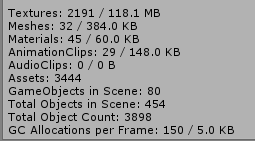
\includegraphics[width=0.3 \textwidth]{04ResultadosObetnidos/imagenes/cutsceneProfiler02.png}}
  \caption{Resultados de la herramienta \textit{profiler} al analizar una cinemática.}
  \label{fig:CutSeceneprofiler}
\end{figure} 

\begin{figure}
  \centering
  
   \subfigure[Vista general del uso del GPU.] {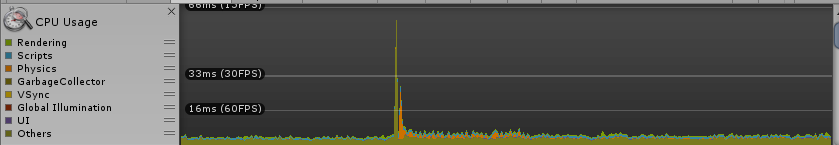
\includegraphics[width=0.6 \textwidth]
   {04ResultadosObetnidos/imagenes/Level02Profiler03.png}}
        
        \subfigure[Desglose de los porcentajes del uso del GPU] {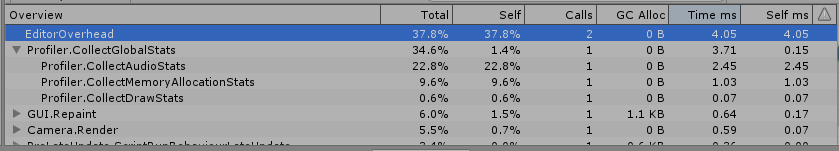
\includegraphics[width=0.6 \textwidth]{04ResultadosObetnidos/imagenes/Level02Profiler04.png}}  
        
        \subfigure[Desglose de los porcentajes del uso de memoria] {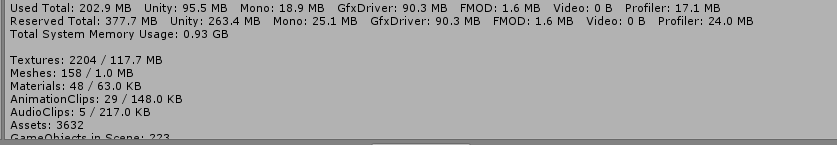
\includegraphics[width=0.6 \textwidth]{04ResultadosObetnidos/imagenes/Level02Profiler08.png}}
  \caption{Resultados de la herramienta \textit{profiler} al analizar un nivel.}
  \label{fig:LevelProfiler}
\end{figure} 
\subsubsection{Conclusiones de la prueba}
Al observar el desglose del uso del GPU en las diferentes escenas que se 
probaron, se identifica al \textit{EditorOverHead} como uno de los principales 
consumidores de recursos; investigando en la documentación de \textit{Unity}, 
se detecta que este elemento es producto de un error de rendimiento en la 
versión 2017 pero que se puede solucionar al descargar uno de los parches que 
\textit{Unity} proporciona desde su sitio web.
\\
\par
Con las pruebas de \textit{profiler} se puede concluir que el juego tiene un buen 
rendimiento en cuanto a uso de recursos puesto que no presenta caídas 
dramáticas en cuanto a desempaño.




